%----------------------------------------------------------------------------------------
\begin{frame}
\begin{center}
\Huge{TOR the Onion router}
\end{center}
\begin{figure}

\includegraphics[width=0.5\linewidth]{./materials/tor.png}
\end{figure}
\end{frame}

%----------------------------------------------------------------------------------------
\begin{frame}
\begin{center}
\frametitle{Onion routing principles}
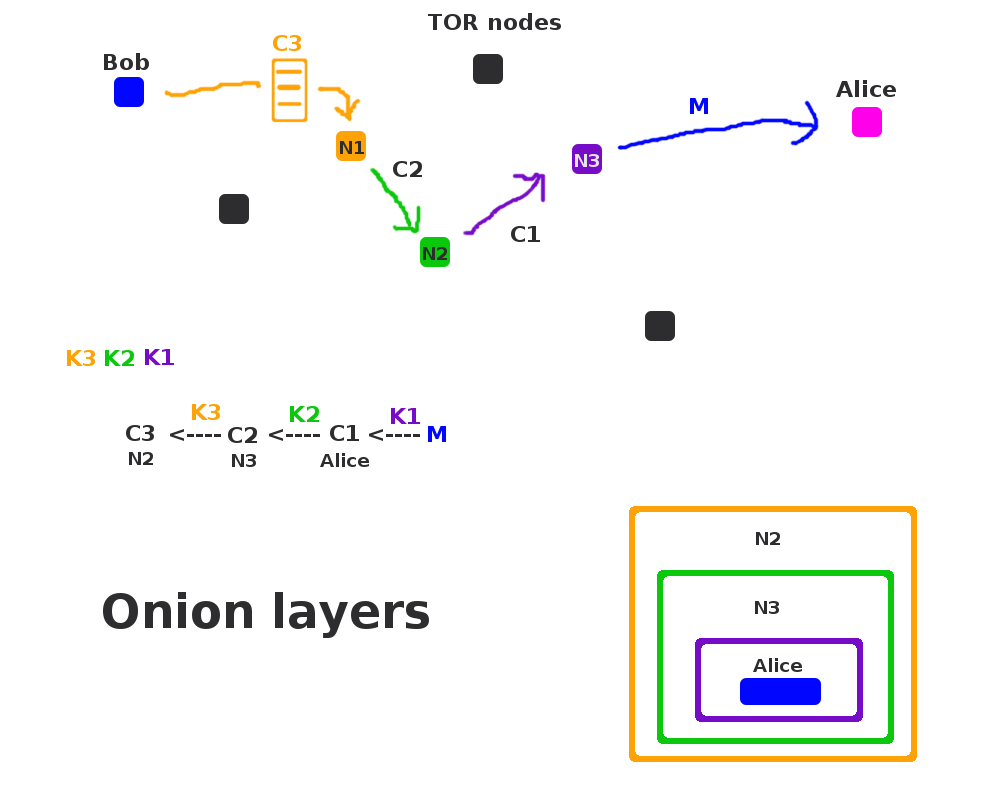
\includegraphics[width=0.8\linewidth]{./materials/Tor_principles_Naam}
\end{center}
\end{frame}

%---------------------------------------------------
\begin{frame}
\frametitle{TOR : The Onion Router}
It's an open-source implementation of the principles we just saw supported by
The Tor Project.
\begin{figure}

\includegraphics[width=0.5\linewidth]{./materials/septical_boy}
\end{figure}
\end{frame}
%---------------------------------------------------
\begin{frame}
\frametitle{TOR : The Onion Router}
\begin{block}{Pros}
\begin{itemize}
\item Hide you identity and location, prevents from eyesdropping.
\item Hide you browsing habits and act like a debrider on the informations that
you're authorized to see.
\item encrypt your (incom|outgo)ing traffic between nodes.
\end{itemize}
\end{block}
\begin{block}{Cons}
\begin{itemize}
\item Slower connexion, forget about downloading big files, torrents
(deanonymize effect) etc...
\item Still vulnerable to some kind of analysis
\\ (timing deduction or infection between applications).
\item entry/exit nodes are vulnerables, no magic here.
\\ (Partial solution if you setup an exit enclaving node)
\end{itemize}
\end{block}
TOR is an anonymity tool, not a security one.
\end{frame}

%---------------------------------------------------
\begin{frame}
\frametitle{If you use it, do it smartly}
\begin{columns}[c]
\column{.5\textwidth}
\begin{itemize}
\item Don't use standalone TOR or Vidalia bundlle
\item Prefer the use of the TBB (Tor Browser Bundle)
\item or even better : tails (live Debian), in hostile environment
(public places etc)
\end{itemize}
\column{.5\textwidth}
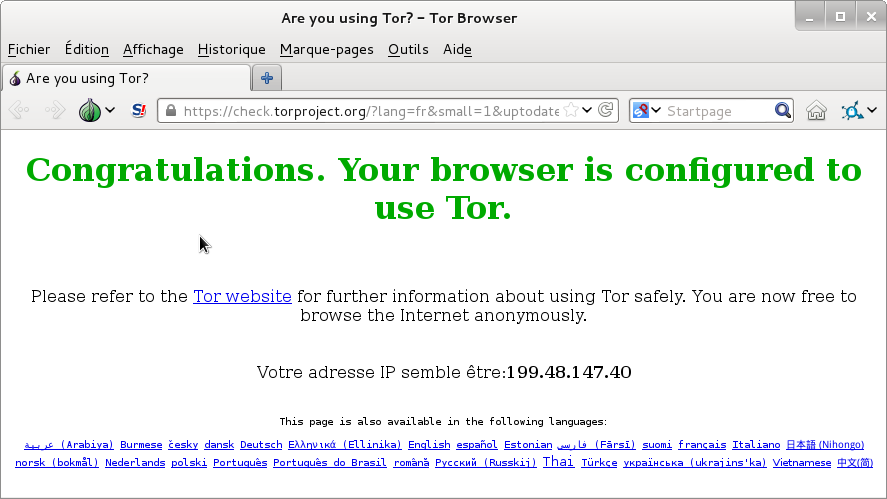
\includegraphics[keepaspectratio,width=\textwidth, height=.8\textheight]{./materials/tbb}
\end{columns}
Try Tor browser launcher for your distribution, that keep TBB updated. Grab-it
from here :\\ https://github.com/micahflee/torbrowser-launcher
\end{frame}
%----------------------------------------------------------------------------------------
\begin{frame}
\begin{center}
\Huge{If it's free, \\then you're the product}
\end{center}
\end{frame}

%----------------------------------------------------------------------------------------
\begin{frame}
\frametitle{What is the tracking?}

\begin{block}{Tracking over the Internet}
\begin{itemize}
\justifying{
\item websites, announcers use it to learn your browsing habits.
\item they save what website are you visiting, what do you like or not and
what you buy.
\item Data are processed in order to display the best ads that fit your
preferences.
}
\end{itemize}
\end{block}
\end{frame}

%----------------------------------------------------------------------------------------
\begin{frame}
\frametitle{What's the magic?}

\justifying{
\begin{block}{Ads and widget are spying you}
\begin{itemize}
\justifying{
\item The Like button : allows FaceBook to know what you visit, even if you
don't click on it, even if you are properly disconnected from Facebook.
\item Same for the +1 by Google, and Google Analytics script.
\item In fact every ads and many widget do it.
}
\end{itemize}
\end{block}
}
\begin{center}

\includegraphics[scale=0.3] {./materials/Facebook_like.png}
\end{center}
\end{frame}

%----------------------------------------------------------------------------------------
\begin{frame}
\frametitle{Want to test? Try LightBeam (ex Collusion) with Firefox}

\justifying{
That add-on allow you to see in real time which websites are tracking you
and the inter-connexion between the actual website and others. Kind of weird
sometime.
}
\begin{center}
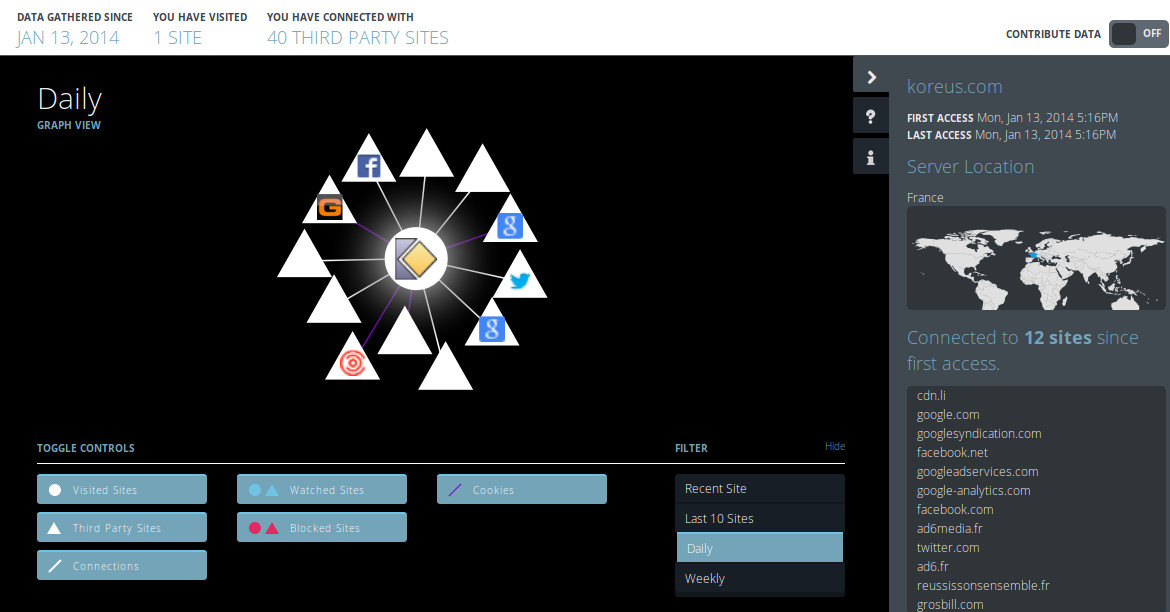
\includegraphics[scale=0.3] {./materials/lightbeam}
\end{center}
\end{frame}


%--------------------------------------------------
\begin{frame}
\frametitle{Firefox}
\begin{center}
\huge{Firefox addons}
\end{center}
\end{frame}

%----------------------------------------------------------------------------------------
\begin{frame}
\frametitle{Firefox scripts : Ghostery}
Block all trackers.\\
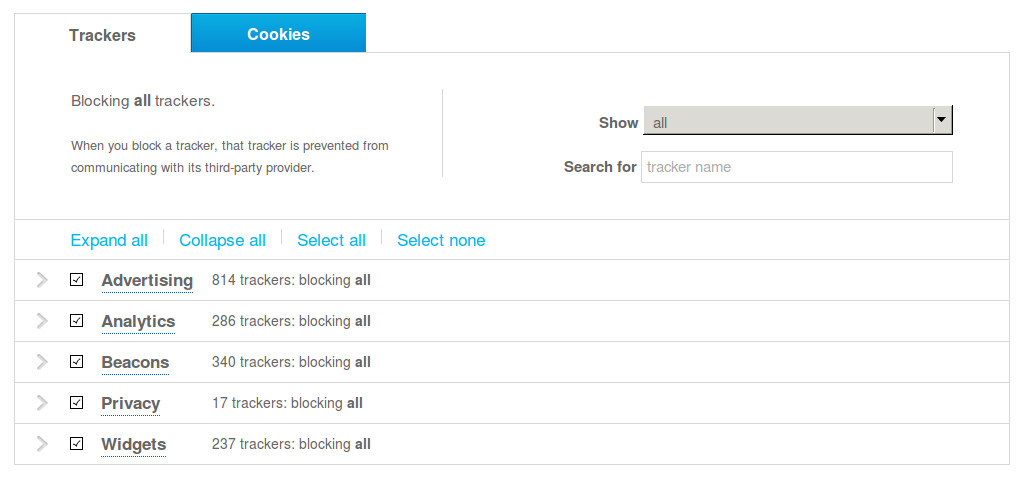
\includegraphics[width=0.9\textwidth]{./materials/ghostery}
\end{frame}

%----------------------------------------------------------------------------------------
\begin{frame}
\frametitle{Firefox scripts : Self destructing cookie}

\begin{columns}[c]
\column{0.5\linewidth}
\justifying{Automatic cookie deletion techniques. Prevent tracking and spying.
Possibility to setup a whitelist if you really want to keep cookie for some
domains even if you're not currently using it.
}
\column{0.5\linewidth}
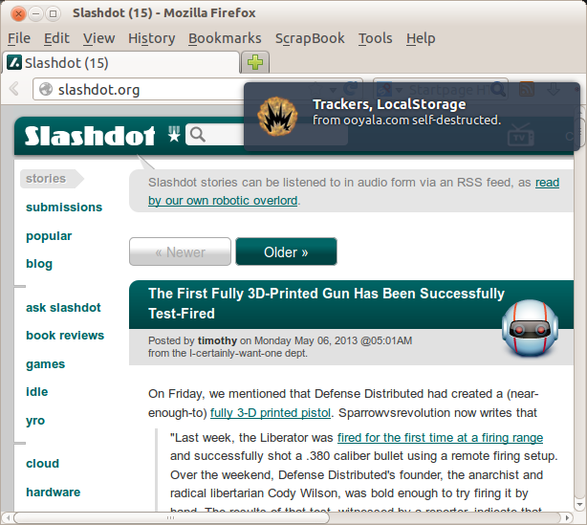
\includegraphics[width=\linewidth] {./materials/selfdestructingcookie.png}
\end{columns}
\end{frame}
%----------------------------------------------------------------------------------------
\begin{frame}
\frametitle{Firefox scripts : HTTPSEverywhere}
\begin{columns}[c]
\column{.5\linewidth}
\justifying{
Made by the electronic frontier fondation (EFF), it force the HTTPS when
available on the website. If you have one, consider registering it for your
visitors (see https://www.eff.org/https-everywhere/rulesets).
\\
Also, activate the SSL Observatory : it prevent from MITM attacks and more
generally against corrupted certificates.
}
\column{.5\linewidth}
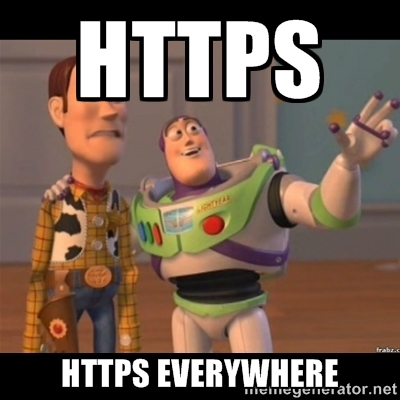
\includegraphics[scale=0.4] {./materials/meme_httpseverywhere}
\end{columns}

\end{frame}
%----------------------------------------------------------------------------------------
\begin{frame}
\frametitle{Firefox scripts : Certificate Patrol}
\justifying{
Does approximately the same thing than the SSLObservatory. Less transparent in
everyday use.
}
\begin{center}
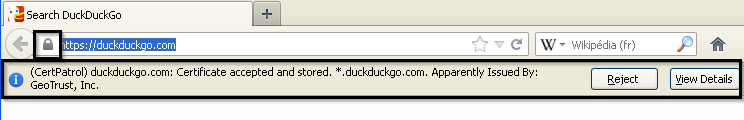
\includegraphics[scale=0.4] {./materials/CertificatePatrol.png}
\end{center}
\end{frame}

%--------------------------------------------------
\begin{frame}
\frametitle{Search engines}
\begin{center}
\huge{Google is not evil... Sure? (PRISM)}
\end{center}
\end{frame}

%----------------------------------------------------------------------------------------
\begin{frame}
\frametitle{Search engines}
\begin{itemize}
\item Duckduckgo (ddg.gg) personalizable interface for your needs.
\item Ixquick/startpage (ixquick.com/startpage.com) more than one search engine
begind, automatic proxy if you want to.
\item binsearch (binsearch.info) search for binaries (newsgroups etc) that
google is hidding from you.
\end{itemize}
\end{frame}

%--------------------------------------------------
\begin{frame}
\frametitle{Metadatas are evil}
\begin{center}
\huge{Metadatas are evil}
\end{center}
\end{frame}

%--------------------------------------------------
\begin{frame}
\frametitle{Metadatas are evil}
\begin{center}
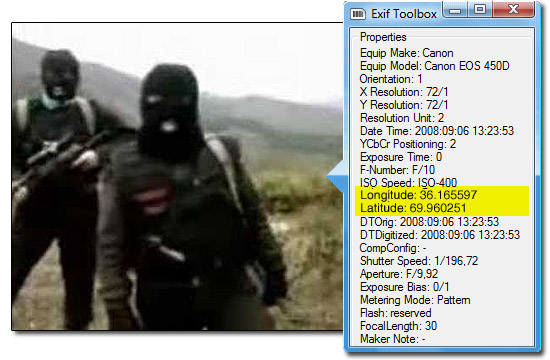
\includegraphics[scale=0.5] {./materials/exif-metadata.jpg} 
\end{center}
\end{frame}

%--------------------------------------------------
\begin{frame}
\frametitle{Metadatas are evil}
\begin{center}
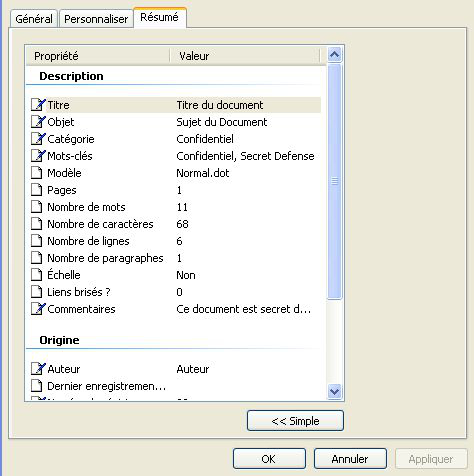
\includegraphics[scale=0.4] {./materials/Word01.jpg} 
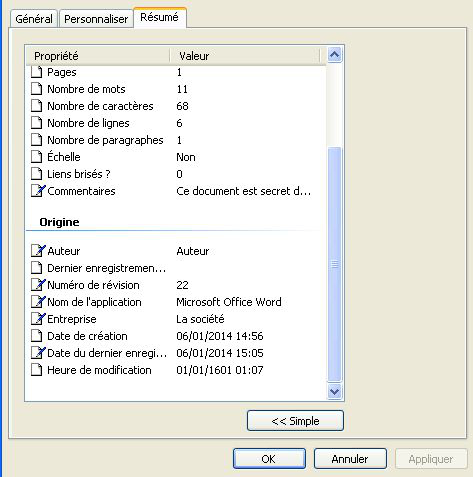
\includegraphics[scale=0.4] {./materials/Word02.jpg} 
\end{center}
\end{frame}

%--------------------------------------------------
\begin{frame}
\frametitle{Metadatas are evil}
\begin{block}{Definition (http://dictionary.reference.com/browse/meta-data)}
\begin{itemize}
\item Data about data.
\item information that is held as a description of stored data.
\end{itemize}
\end{block}
\begin{block}{Examples}
\begin{itemize}
\item EXIF tags on photography (Date, cameras info, GPS coordinates...)
\item data stored on documents like .doc(x)
\item ...
\end{itemize}
\end{block}
\end{frame}


%--------------------------------------------------
\begin{frame}
\frametitle{Metadatas are evil}
\begin{center}
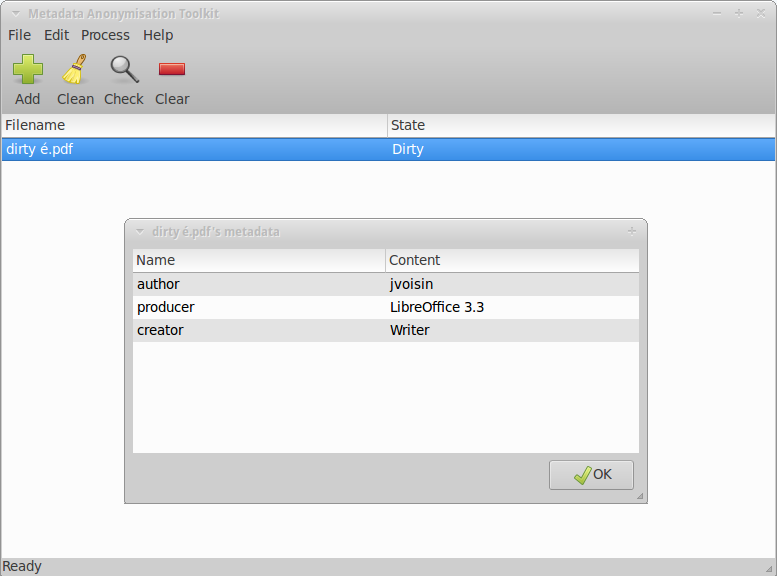
\includegraphics[scale=0.4] {./materials/Mat.png} 
\end{center}
\end{frame}

%--------------------------------------------------
\begin{frame}
\frametitle{Solution? YES, partialy}
There is a good tool to erase metadatas from a large spectrum of filetypes.
It's called MAT (mat.boum.org).
\begin{itemize}
\item Reside in Tails, standalone package (Debian), Git repos.
\item it has a GUI, no worry (can also be used in command line, don't
 worry too).
\end{itemize}
Files support :
\begin{itemize}
\item Images : .png, JPEG (.jpg, .jpeg, …)
\item Documents : .odt, .odx, .ods, …, .docx, .pptx, .xlsx, …, .pdf
\item Tape ARchives (.tar, .tar.bz2, …)
\item Media : .mp3, .mp2, .mp1, …, .ogg, …, .flac
\item Torrent (.torrent)
\end{itemize}
\end{frame}
